%
% PROTOCOL AND FUNCTIONALITY
%
\JWltwo{OPE Protocol \& Functionality}
\label{sec:protocol}

\JWtodo{Hier fehlt wahrscheinlich noch etwas Beschreibung was das ist}

This chapter defines the functionality \JWfuncSymOPE and the protocol
\JWprotoSymOPE this thesis proposes to realize the functionality. The
functionality (described in figures \ref{fig:func-ope} and \ref{fig:graph-ope})
is the ideal model of what the protocol tries to achieve.

\begin{JWfunc}%
  {\JWfuncSymOPE}%
  {The ideal $\JWfieldGeneral{}$-OPE functionality \JWfuncSymOPE{}}%
  {fig:func-ope}

  Parametrized by a finite field of size $2^k$ ($\mathbb{F}_{2^k}$)
  and polynomial degree $n$.

  \begin{JWfuncSteps}

  \item Upon receiving input \JWmsgTP{Commit}{$a$} from the environment, verify
    $a \in \JWfieldGeneral^{n+1}$ and that there is no stored input, yet; else
    ignore that input. Next record $a$.

  \item Upon receiving input \JWmsgTP{Evaluate}{$x$} from the environment,
    verify $x \in \JWfieldGeneral{}$ and that there is no stored input, yet;
    else ignore that input. Next record $x$.

  \item Upon $a$ and $x$ are verified and stored, compute $y \leftarrow
    \sum_{i=0}^n a_ix^i$ and output \JWmsgTP{Evaluated}{$y$}.

  \end{JWfuncSteps}
\end{JWfunc}

\begin{figure}[ht]

  \centering

  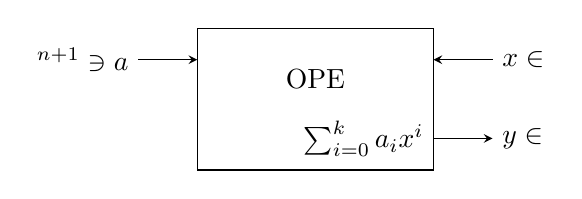
\begin{tikzpicture}[>=stealth]

    \node (OPE) at (8.5,0) {OPE};
    \draw (OPE) +(-1.5,-1.15) rectangle +(1.5,0.65);

    \draw [<-] (OPE) ++(-1.5,0.25) node [anchor=west] {} -- +(-0.75,0) node
    [anchor=east] {$\JWfieldGeneral^{n+1} \ni a$};

    \draw [<-] (OPE) ++(1.5,0.25) node [anchor=east] {} -- +(0.75,0) node
    [anchor=west] {$x \in \JWfieldGeneral$};

    \draw [->] (OPE) ++(1.5,-0.75) node [anchor=east] {$\sum_{i=0}^k a_ix^i$}
    -- +(0.75,0)
    node [anchor=west] {$y \in \JWfieldGeneral$};

  \end{tikzpicture}

  \caption{Graphical Representation of \JWfuncSymOPE}
  \label{fig:graph-ope}

\end{figure}

\begin{JWprotocol}%
  {\JWprotoSymOPE}%
  {Protocol: Oblivious Polynomial Evaluation}%
  {fig:proto-ope}

  Parametrized by the security parameter $k$ that specifies the field
  $\mathbb{F}_{2^k}$ and the degree of the polynomial $n$.

  \JWprotoPhase{Setup:}

  \begin{JWprotoSteps}

  \item Upon input \JWmsgTP{Commit}{$a$} from the environment, \JWpOne{}
    verifies that $a \in \mathbb{F}_{2^k}^{n+1}$; else ignore that input. Next,
    \JWpOne{} generates the DRAC and sets up the OAFE functionality for the
    polynomial $f(x) = \sum_{i=0}^n a_ix^i$ (see section \ref{sec:OPE}).

  \item Finally, \JWpOne{} sends the DRAC to \JWpTwo{}.

  \end{JWprotoSteps}


  \JWprotoPhase{Evaluation:}

  \begin{JWprotoSteps}

  \item Upon receiving the DRAC from \JWpOne{}, verify that there is no stored
    DRAC yet, else ignore that input. Next, \JWpTwo{} verifies the received
    input is a DRAC, else ignore that input. Additionally it verifies
    that the DRAC encodes a function whose degree is equal to $n$ (see
    chapter \ref{sec:max-poly-degree}), else ignore the input. If the DRAC
    verification was successful, store the DRAC.

  \item Upon receiving input \JWmsgTP{Evaluate}{$x$} from the environment,
    verify that $x \in \mathbb{F}_{2^k}$, else ignore that input. If there is
    already a stored DRAC, continue at the next step, else wait for a stored
    DRAC.

  \item Next, \JWpTwo{} evaluates the DRAC. Because the OAFE functionality is
    set up by \JWpOne{}, during the evaluation it is possible that the OAFE
    functionality turns out to behave unexpectedly: It could decline needed
    evaluations and it could return vectors of unexpected shapes. In both cases
    always assume it would have returned all zero vectors of the expected shape.

  \item After the evaluation, \JWpTwo{} adds both components of the last DRAV
    and queries a special final OAFE with that value. Again, assume the all zero
    vector if the OAFE behaves unexpectedly. The then received new value is the
    result of the computation $y = \sum_{i=0}^k a_ix^i$. Finally, output
    \JWmsgTP{Evaluated}{$y$} to the environment.

  \end{JWprotoSteps}

\end{JWprotocol}

% vim: set spell spelllang=en_us fileencoding=utf8 :
